\subsubsection{Implementation}
To adapt the trivial recursive implementation to use cilk, only two new keywords have to be added to the calling code of the recursions:

\textbf{Recursive calls:}
\begin{lstlisting}
  cilk\_spawn fft_help(dc2, dc1, len, step*2);
  cilk\_spawn fft_help(dc2+step, dc1+step, len, step*2);
  cilk\_sync;
\end{lstlisting}

cilk\_spawn tells cilk that the function call (here the recursive calls to fft\_help) can be executed in parallel to the calling function. It is important to note that while the cilk\_spawn keyword permits parallelism, it does not explicitly create a thread. It tells the runtime that the part after the keyword can be executed by another worker. 

cilk\_sync  tells the runtime that all child functions spawned until this point must be completed before the execution can continue past this point. In our case this means that both recursive calls must be completed before the program can continue. 

\textbf{Cutoff}
In addition to the trivial parallelism we also implemented a cutoff threshold after which the remaining parts of the fft will be executed sequentially. 

This can be seen here (with sequential being the same recursive funtion, without the cilk\_ statements: 
\begin{lstlisting}
if((len/2)/step < 64) { //cutoff
		sequential(dc1, dc2, len, step);
		return;
	}
\end{lstlisting}

\subsubsection{Performance}

Average speedup:

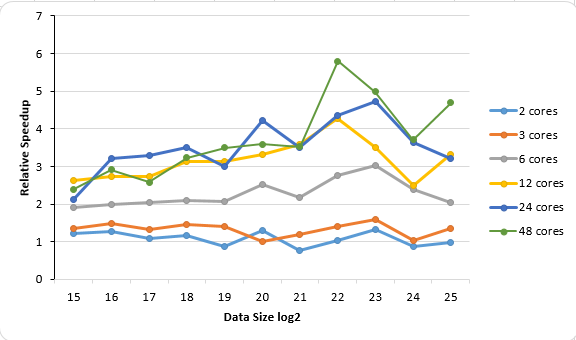
\includegraphics[width=\textwidth]{cilk_rec_avg.png}

Best observered speedup:

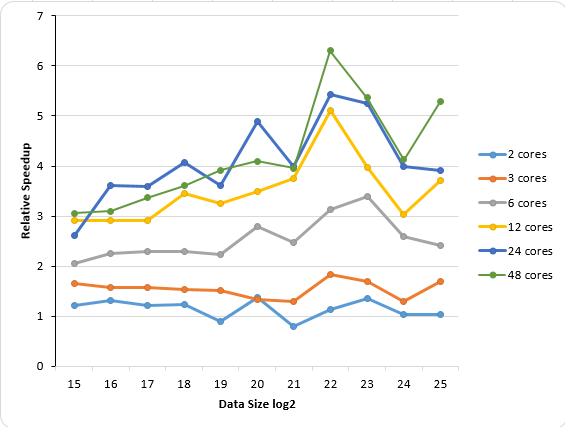
\includegraphics[width=\textwidth]{cilk_rec_best.png}

The graphs again show the same pattern for the speedup, that was already present for both OpenMP implementations, but with a few noticable differences.

First of all the corellation between data size and speedup for larger amounts of cores seems to be lower. We assume this is due to the cutoff having less of an ill effect in the cilk runtime, since even before we get to this point there may already have been parts of the fft executed sequentially, due to the way the cilk\_spawn keyword works. 

Furthermore there is less of a noticable difference speedup between the higher amounts of cores (especially between 24 and 48 cores). We did not find a plausible reason for this in our implementation, but we suspect it might be due to the cilk runtime on the testing server running into problems with higher ammount of cores. This suspicion is supported by the fact that running the cilk program on the server led to high amount of system cpu time used on all cores, while only one core was doing work, which can be seen in the following screenshot: 

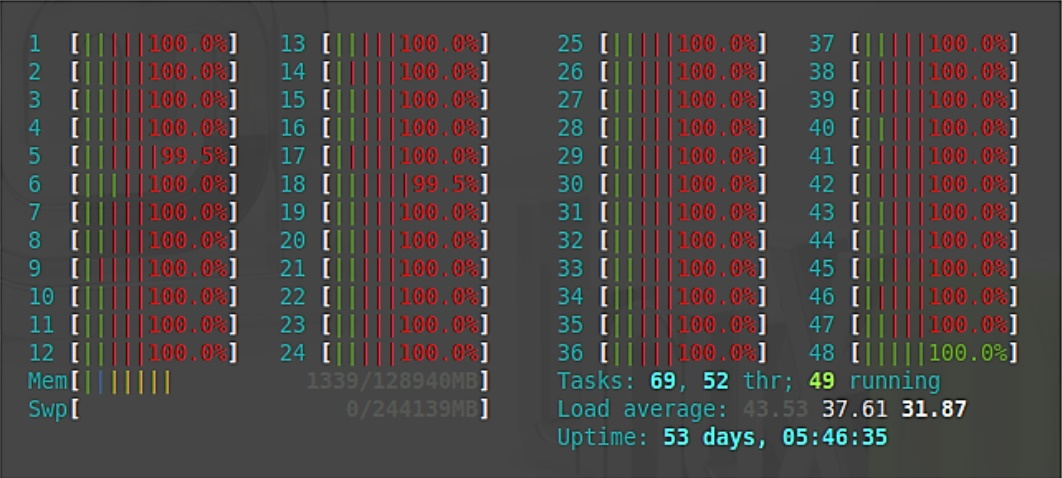
\includegraphics[width=\textwidth]{cpu_util_cilk.jpg}
